\documentclass[13.5pt]{beamer}
\usepackage[natbib=true,backend=bibtex,useprefix=true]{biblatex}
\usepackage[utf8]{inputenc}
\usepackage{tikz}
\usepackage{ragged2e}
\usepackage{adjustbox}
\usepackage{amsmath}
\usepackage{amsfonts}
\usepackage{amssymb}
\usepackage{amsthm}
\usetikzlibrary{fadings}
\usepackage{fontspec}
\usepackage{unicode-math}
\setmathfont{XITS Math}


\usetheme{Madrid}

\definecolor{TorVergataColor}{RGB}{0,125,52}
\setsansfont[BoldFont={Circe-Bold}]{Circe-Regular}

\newcommand{\B}[1]{\textcolor{TorVergataColor}{\textbf{#1}}}
\newcommand{\Cross}{\mathbin{\tikz [x=2.5ex,y=2.5ex,line width=.10ex] \draw (0,0) -- (1,1) (0,1) -- (1,0);}}
\newcommand{\mathDef}{\overset{\textit{def}}{=}}
\newcommand{\N}{\mathbb{N}}
\newcommand{\R}{\mathbb{R}}
\newcommand{\Rplus}{\mathbb{R}^+}

\makeatletter
\setbeamertemplate{title page}{%
	\vbox{}
	\vfill
	{\usebeamercolor[fg]{titlegraphic}\inserttitlegraphic\par}
	\begingroup
	\centering
	\begin{beamercolorbox}[sep=8pt,center]{title}
		\usebeamerfont{title}\inserttitle\par%
		\ifx\insertsubtitle\@empty%
		\else%
		\vskip0.25em%
		{\usebeamerfont{subtitle}\usebeamercolor[fg]{subtitle}\insertsubtitle\par}%
		\fi%     
	\end{beamercolorbox}%
	\vskip1em\par
	\vfill%<- added
	\begin{beamercolorbox}[sep=8pt,left]{author}
		\usebeamerfont{author}\insertauthor
	\end{beamercolorbox}
	\vfill%<- added
	\begin{beamercolorbox}[sep=8pt,center]{institute}
		\usebeamerfont{institute}\insertinstitute
	\end{beamercolorbox}
	\vfill%<- added
	\begin{beamercolorbox}[sep=8pt,center]{date}
		\usebeamerfont{date}\insertdate
	\end{beamercolorbox}%
	\vskip0cm%<- changed
	%    
	\endgroup
	\vfill%<- removed
}
\makeatother



\setbeamercolor{structure}{fg=TorVergataColor}
\setbeamerfont{structure}{family=\bfseries,size=\large}

\title[]
{ 
	\textbf{A QoS-Aware Broker \\ for Multi-Provider Serverless Applications}
}

\author[Andrea Graziani (m. 0273395)]{{\Large \textbf{Andrea Graziani}}\\m. $0273395$\\[10mm]{\small 
		\begin{tabular}{l|l}
			\textbf{Supervisor}: & \textit{Valeria Cardellini } \\ 
			\textbf{Tutor}: & \textit{Gabriele Russo Russo}  \\  
\end{tabular}}}

\titlegraphic{
\includegraphics[width=9.5cm,height=2.4cm]{../Images/UniLogo/LogoMacroarea.png}}

\setbeamertemplate{background}{%
	\begin{tikzpicture}[overlay,remember picture]
		\node[scope fading=west,anchor=north west] at ([shift={(2in,-1in)}]current page.north west) {
\includegraphics[width=9cm,height=9cm]{../Images/UniLogo/TorVergataWatermark.png}};
	\end{tikzpicture}
}

\justifying

\setbeamertemplate{frametitle}{%
	\nointerlineskip%
	\begin{beamercolorbox}[wd=\paperwidth,ht=4.0ex,dp=1ex]{frametitle}
		\hspace*{1ex}\insertframetitle%
	\end{beamercolorbox}%
}

\addtobeamertemplate{frametitle}{}{%
	\begin{tikzpicture}[remember picture,overlay]
		\node[anchor=north east,yshift=2pt] at (current page.north east) {
\includegraphics[height=1cm]{../Images/UniLogo/NegativeTorVergataLogo.png}};
\end{tikzpicture}}

\date{May 23, 2022}

%-------------------------------------------------------
% THE BODY OF THE PRESENTATION
%-------------------------------------------------------

\begin{document}

%-------------------------------------------------------
% THE TITLEPAGE
%-------------------------------------------------------

{% % this is the name of the PDF file for the background
\begin{frame}[plain,noframenumbering] % the plain option removes the header from the title page, noframenumbering removes the numbering of this frame only
  \titlepage % call the title page information from above
\end{frame}}

\setbeamertemplate{background}{}

% -------------- %
% -------------- %
\begin{frame}{Goals}
% -------------- %
% -------------- %

\begin{block}{}
	\centering
	My thesis is focused on ``\B{Serverless Computing}".
\end{block}

\vspace{\baselineskip}
Two main goals:
\begin{enumerate}
	\item The \B{orchestration} of a serverless workflow supporting:
	
	\begin{itemize}
		\item \textbf{Multiple FaaS Providers}
		\item \textbf{Multiple Functions Implementations.}
	\end{itemize}
	\vspace{\baselineskip}
	\item The fulfillment of \B{non-functional requirements} concerning the \B{quality of service} (QoS) levels that should be guaranteed.
\end{enumerate}

\end{frame}
% -------------- %
% -------------- %
\begin{frame}{Serverless Computing: Overview}


\begin{block}{}
\centering
What's meant by serverless computing?
\end{block}
\vspace{\baselineskip}
An applications service model where:
\vspace{\baselineskip}
\begin{itemize}
	\item Administration tasks (provisioning, monitoring, scaling, etc.) are directly managed by the provider.
	\vspace{\baselineskip}
	\item Small-granularity billing pricing model: \B{pay-as-you-go}.
	\vspace{\baselineskip}
	\item Cloud application are abstracted as a group of so-called \\ ``\B{Serverless Functions}".
\end{itemize}

\end{frame} 
% -------------- %
% -------------- %
\begin{frame}{Serverless Computing: Overview}
	
	\begin{block}{}
		\centering
		What is a serverless function?
	\end{block}
	\vspace{\baselineskip}
	A computation unit implementing a business functionality.
	
	\begin{itemize}
		\item \B{Stateless}
		\item \B{Event-Driven}
		\item \B{Short-Lived}
	\end{itemize}

	\vspace{\baselineskip}
	
	\begin{block}{Serverless Application}
		\justifying
		A software system made up of a serverless functions set.
	\end{block}

\end{frame} 
% -------------- %
% -------------- %
\begin{frame}{Serverless Computing: Overview}
	
	\begin{block}{}
		\centering
		A serverless function is executed inside a containerized environment: the so-called ``\B{Function Instance}".
	\end{block}
	\vspace{\baselineskip}
	
	\begin{block}{}
		\centering
		The FaaS platform \B{automatically} scales the number of function instances.
	\end{block}
	
	\vspace{\baselineskip}
	When a request comes in, only one of the following events can occur:
	\begin{itemize}
		\item \textbf{Warm start}.
		\item \textbf{Cold start.}
	\end{itemize}
	
	
\end{frame} 
% -------------- %
% -------------- %
\begin{frame}{Serverless Computing: Overview}
	
	\begin{block}{Concurrency Level}
		The limitation, imposed by FaaS platforms, on the \B{number} of function instance runnable at the \B{same time}.
	\end{block}
	\vspace{\baselineskip}
	Providers apply that restriction differently:
	\vspace{\baselineskip}
	\begin{itemize}
		\item \B{Global (Per-Account) Concurrency Model}.
		\begin{itemize}
			\item AWS Lambda. 
			\item IBM Cloud Functions.
		\end{itemize}
		\vspace{\baselineskip}
		\item \B{Local (Per-Function) Concurrency Model}.
		\begin{itemize}
			\item Google Cloud Functions.
		\end{itemize}
	\end{itemize}

\end{frame} 
% -------------- %
% -------------- %
\begin{frame}{Serverless Computing: Overview}
	
	\begin{block}{}
		\centering
		To invoke a \B{serverless function}, users have to specify a so-called \B{serverless function configuration}.
	\end{block}
	\vspace{\baselineskip}
	\begin{block}{}
		\centering
		To invoke a \B{serverless application}, users have to specify a configuration for \B{all} its functions.
	\end{block}
	
	
\end{frame} 
% -------------- %
% -------------- %
\begin{frame}{Serverless Computing: Overview}
	
	Configuration parameters \B{significantly} affect the \B{cost} and \B{response time} of serverless functions.
	\vspace{\baselineskip}
	\begin{figure}[h]
		\centering
		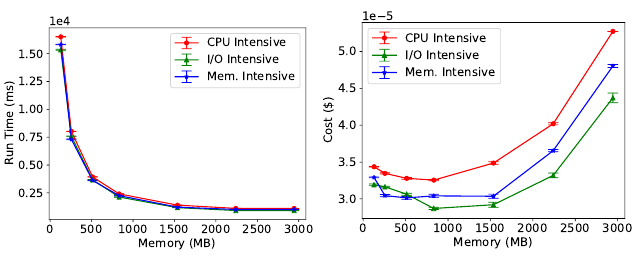
\includegraphics[width=\textwidth]{../Images/slideImage1.png}
	\end{figure}
	
\end{frame} 
% -------------- %
% -------------- %
\begin{frame}{Serverless Computing: Problems}
	
	\begin{block}{}
		\centering
		What current problems or limitations of the serverless computing paradigm I tried to solve?
	\end{block}
\vspace{\baselineskip}
	\begin{itemize}
		\item No support for application whose functions are hosted on multiple providers.
		\item No support for application whose functions have more than one implementation (\B{Concrete Functions}).
		\item Vendor lock-in issues.
		\item The fulfillment of quality of service (\textit{QoS}) levels.
	\end{itemize}

\end{frame} 
% -------------- %
% -------------- %
\begin{frame}{Serverless Computing: Problems}
	
	\begin{block}{}
		\centering
		Why is so difficult to guarantee QoS levels?
	\end{block}
	\vspace{\baselineskip}
	\begin{itemize}
		\item Lack of an analytical model to predict application performance.
		\vspace{\baselineskip}
		\item Lack of a methodological way to find a suitable configuration for a serverless application.
	\end{itemize}

\end{frame} 

% -------------- %
% -------------- %
\begin{frame}{Related Works}

Solutions \B{already} exist, but:
\vspace{\baselineskip}
\begin{itemize}
	\item They are unaware of the current status of FaaS platforms.
	\item No support for Multi-Provider, Multiple-Implementations serverless applications. 
	\item Many do not support generic workload applications.
\end{itemize}

\end{frame} 

% -------------- %
% -------------- %

\begin{frame}{My Contributions}
	
	My contributions respect to the current state of art:
	\vspace{\baselineskip}
	\begin{enumerate}
	
		\item An \B{Analytical Model} to evaluate applications performance.
		\begin{itemize}
			\item Supports generic workflow (branch, loop, parallel)
			\item Multi-Provider support.
			\item Support for Multi-Implementation for functions.
			\item FaaS-Status-Aware.
		\end{itemize}
		\vspace{\baselineskip} 
		\item A \B{Methodological Way} to find the ``best" configuration to satisfy QoS constraints.
		\begin{itemize}
			\item By solving an \B{Optimization Problem} (LP).
		\end{itemize}
		\vspace{\baselineskip} 
		
	\end{enumerate}
	
\end{frame} 

% -------------- %
% -------------- %

\begin{frame}{My Contributions}
	
	\vspace{\baselineskip}
	\begin{enumerate}
		\justifying
		\setcounter{enumi}{2}
		\item A custom \B{Heuristic Algorithm} to resolve the aforementioned optimization problem.
		\begin{itemize}
			\item Based on \B{Ant Colony Optimization} algorithm (ACO) family.
		\end{itemize}
		\vspace{\baselineskip} 
		\item A \B{QoS-Aware Software Framework} for the orchestration for multi-provider, multiple-implementations serverless applications. 
		
		\vspace{\baselineskip} 
		\item An extension to an already existent \B{Representation Scheme} to define a serverless application workflow.
		\begin{itemize}
			\item Based on an existing language called \B{Abstract Function Choreography Language} (AFCL).
		\end{itemize}
		
	\end{enumerate}
	
\end{frame} 

% -------------- %
% -------------- %

\begin{frame}{The Prototype}
	
 	Main features of our software framework:
	\vspace{\baselineskip}
	\begin{itemize}
		\item \B{Client-Server architecture}.
		\item \B{Cloud-native} application.
		\item Includes a set of \B{adapters} to interact with following FaaS providers:
		\begin{itemize}
			\item AWS Lambda.
			\item Apache OpenWhisk.
		\end{itemize}
		\item \B{REST} architectural style.
	\end{itemize}
	
\end{frame} 
% -------------- %
% -------------- %
\begin{frame}{The Prototype}
	
	Main logical entities of our system:
	
	\begin{itemize}
		\item A Logging subsystem.
		\item An Orchestrator.
		\item A profiler.
		\item A QoS-aware model-based optimizer.
		\item A Custom AFCL Parser.
	\end{itemize}
	
\end{frame} 

% -------------- %
% -------------- %
\begin{frame}

\begin{figure}[h]
	\centering
	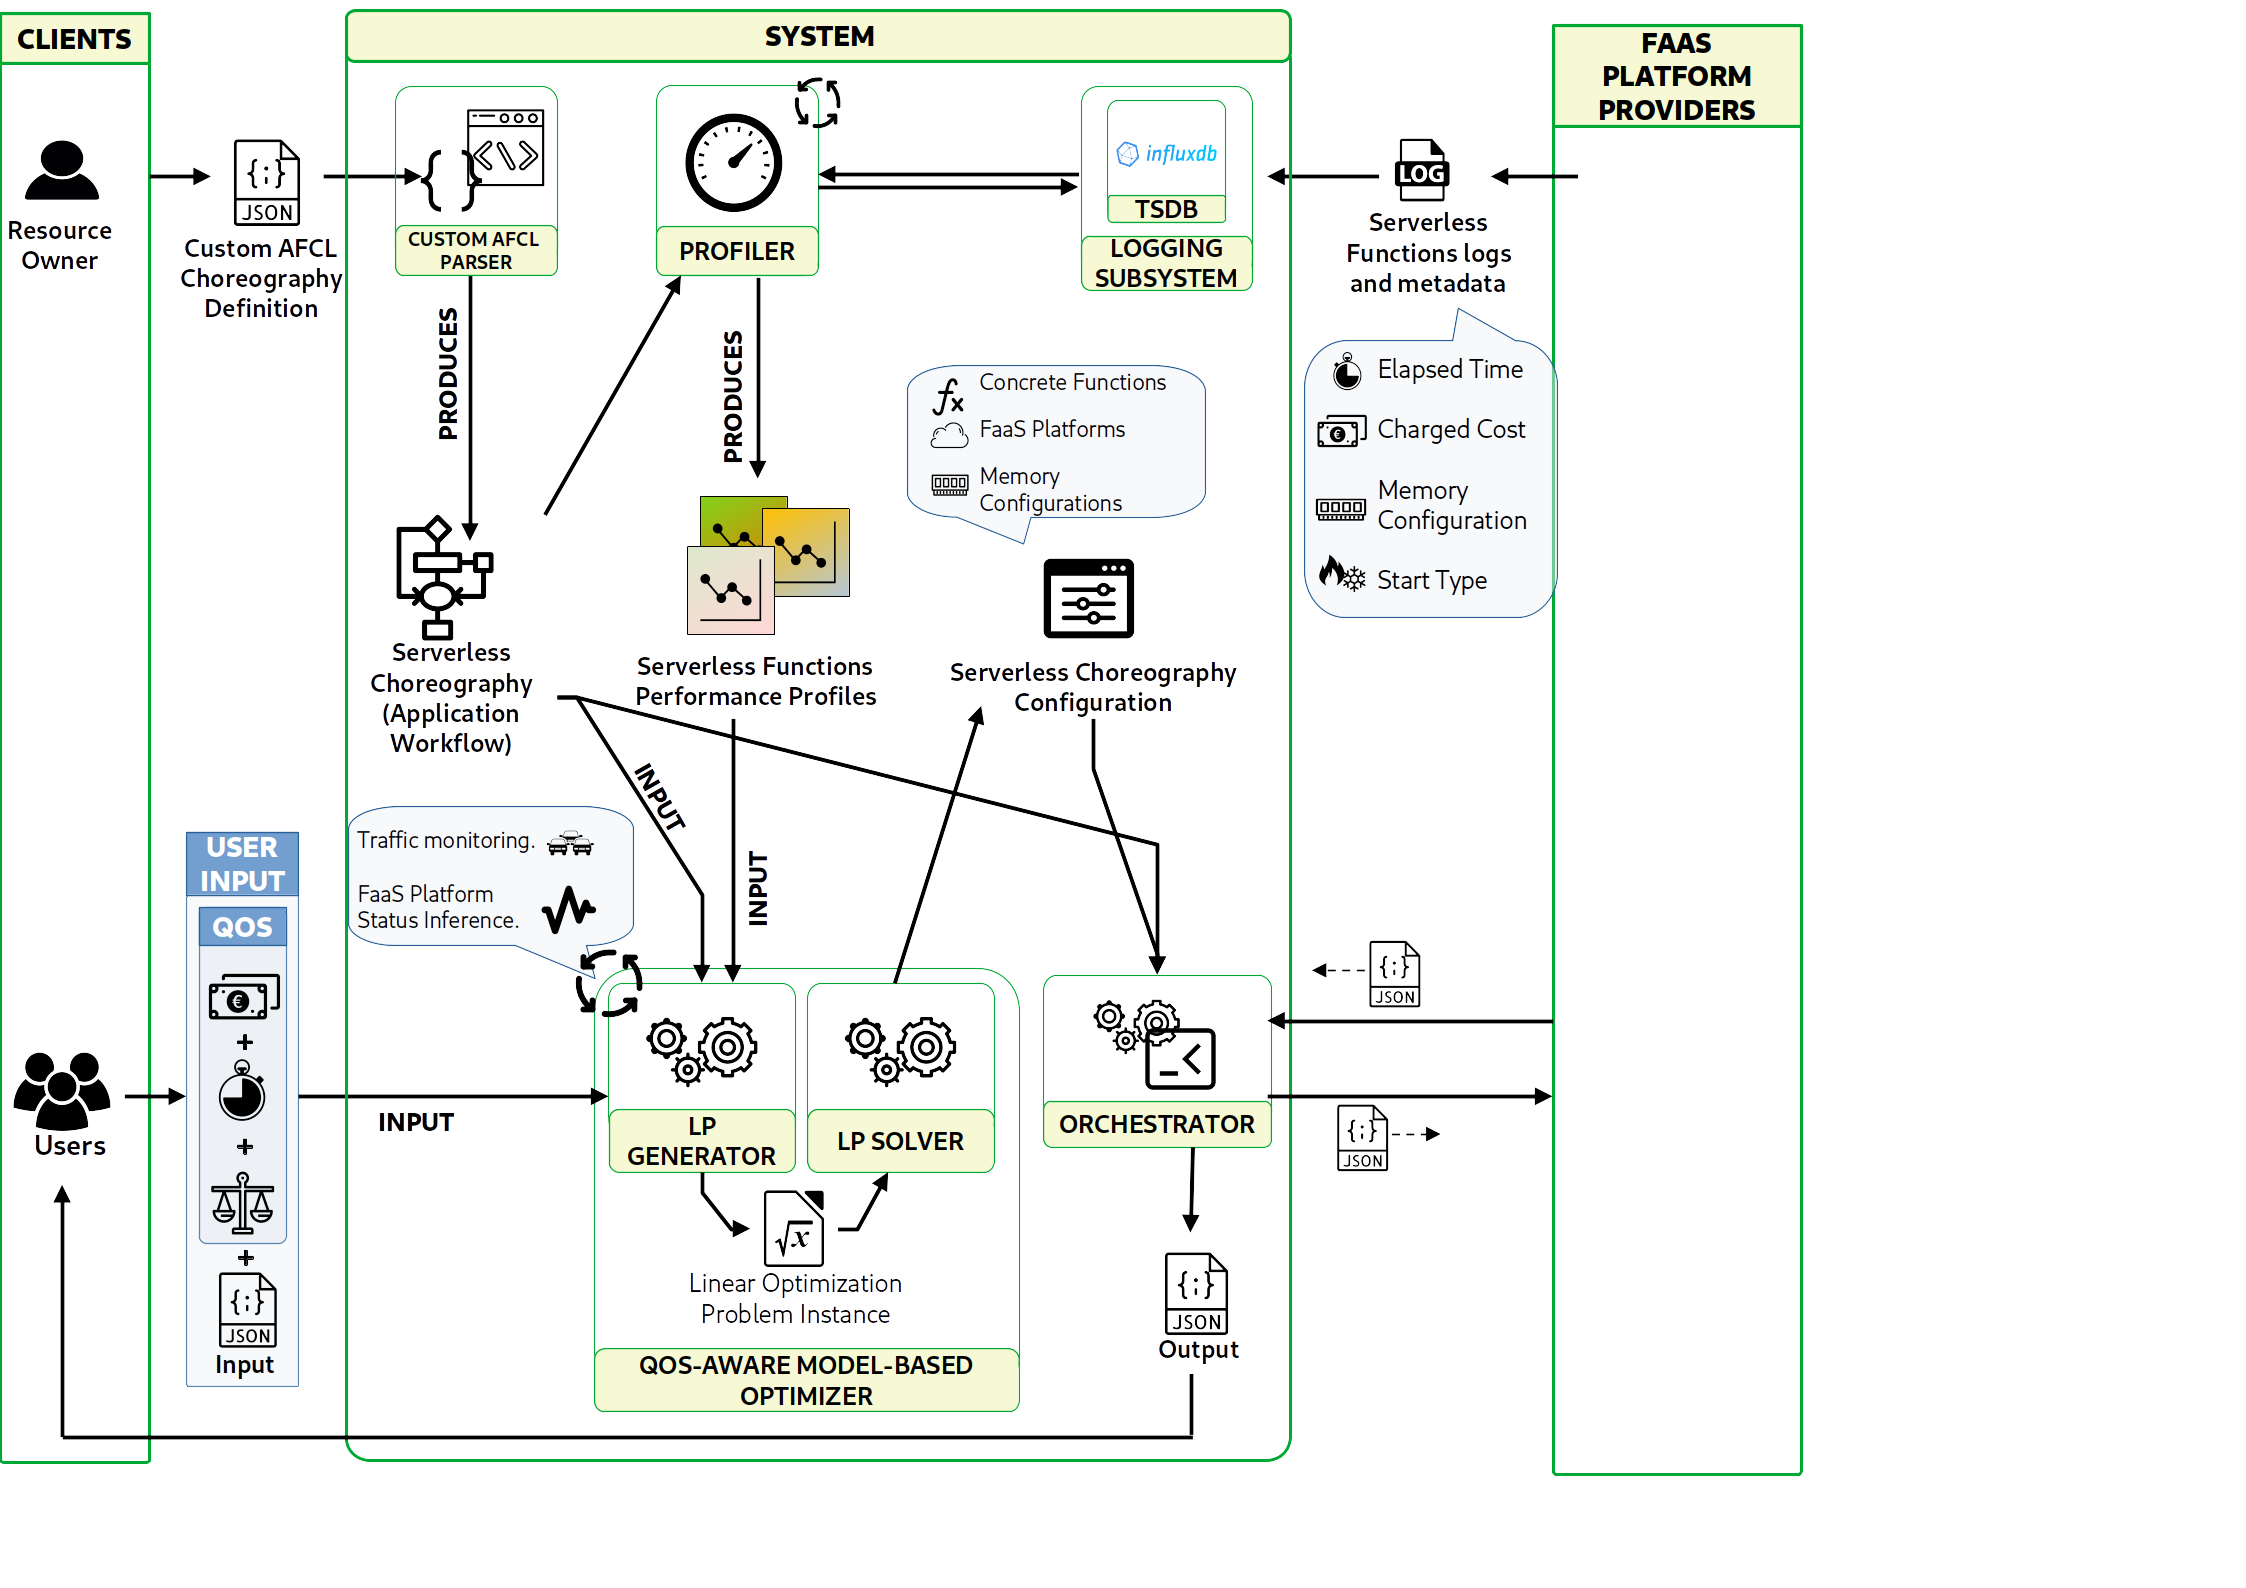
\includegraphics[width=\textwidth]{../Images/SystemForSlide.png}
\end{figure}


\end{frame} 
% -------------- %
% -------------- %
\begin{frame}{The Prototype}
	
	\begin{block}{}
		\centering
		The use of an unique representation scheme for serverless workflows \B{mitigates portability limitations and vendor lock-in issues}.
	\end{block}

	\vspace{\baselineskip}

	\begin{block}{}
		\centering
		Serverless application are managed using identical operations based on standard \texttt{HTTP} methods providing \B{Access Transparency}.
	\end{block}

\end{frame} 
% -------------- %
% -------------- %
\begin{frame}{The Analytical Model}
	
	\begin{block}{}
		\centering
		Serverless applications are abstracted to a \\\B{Weakly Connected Weighted Directed Graph}.
	\end{block}
	\vspace{\baselineskip}
	\begin{itemize}
		\item Each \B{vertex} models an \B{abstract serverless function}, that is a computational unit required by business logic.
		\begin{itemize}
			\item To each abstract function corresponds a set containing all concrete function implementing it.
		\end{itemize}
		\vspace{\baselineskip}
		\item Each \B{edge} represents the calling relationship between two abstract functions.
		\begin{itemize}
			\item Edge weights represent the so-called \B{transition probability}. 
		\end{itemize}
	\end{itemize}
	
	

	
\end{frame} 
% -------------- %
% -------------- %
\begin{frame}{The Analytical Model}

To evaluate the performance of a \textbf{Concrete Function}:
\vspace{\baselineskip}
\begin{itemize}
	\item Estimations about the \B{Average Response Time} (\B{Cost}) in case of cold (warm) start are required.
	\begin{itemize}
		\item To compute aforementioned estimations, \B{Exponential Moving Average} based approach is adopted.
	\end{itemize}
	\vspace{\baselineskip}
	\item An estimation of the probability according to which a request follows a cold start (\B{Cold Start Probability}) is required.
\end{itemize}

\end{frame} 
% -------------- %
% -------------- %
\begin{frame}{The Analytical Model}
	
	To compute \B{Cold Start Probability}:
	
	\begin{itemize}
		\vspace{\baselineskip}
		\item Any FaaS platform provider is modeled  by \B{set} of $M/G/K(t)_{\textbf{C}_{max}}/K(t)_{\textbf{C}_{max}}$ queueing systems.
		\begin{itemize}
			\item $K(t)$: the number of function instances at time $t$.
			\item $C_{max}$: the concurrency limit.
		\end{itemize}
		\vspace{\baselineskip}
		\item Aforementioned set depends on the concurrency model adopted by providers.
		\vspace{\baselineskip}
		\item \B{Erlang-B} formula is used.
	\end{itemize}
	
	
	
\end{frame}
% -------------- %
% -------------- %
\begin{frame}{}
	
\begin{figure}[h]
	\centering
	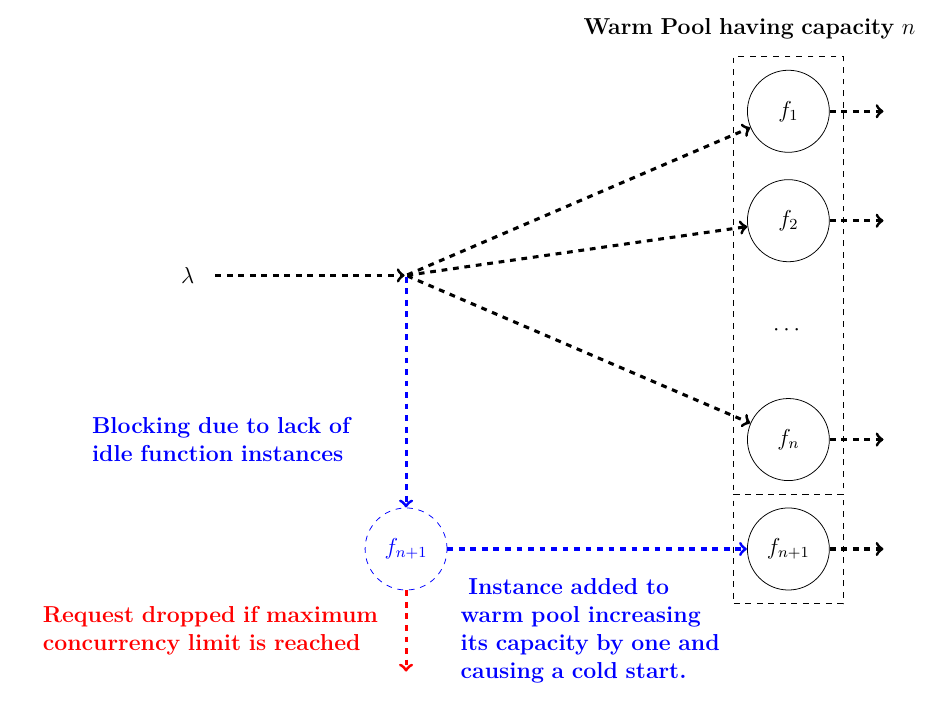
\includegraphics[width=\textwidth]{../Images/FaaSForSlide.png}
\end{figure}
	
\end{frame} 
% -------------- %
% -------------- %
\begin{frame}{The Analytical Model}
	

\begin{block}{}
	I formalized algorithms and equations to evaluate the performance of both a \B{serverless application} and of an \B{abstract function}.
\end{block}
\vspace{\baselineskip}

Aforementioned algorithm depends on:
\begin{itemize}
	\item The topological properties of the graph representing the application.
	\item The actual value of transition probabilities of all edges.
\end{itemize}

\end{frame}
% -------------- %
% -------------- %
\begin{frame}{The Optimization Problem}

\begin{itemize}
	\item To achieve our goal consisting in finding the best configuration to guarantee QoS constraints, we have to solve an \B{optimization problem}.
	\begin{itemize}
		\item It is based on \B{Multi-Dimensional Multi-Choice Knapsack Problem Formulation}. 
	\end{itemize}
\end{itemize}

\end{frame}


\begin{frame}{The Optimization Problem}
	Formally, the configuration vector $\textbf{x}_{\mathcal{C}}$ we want to find is such that:
	
	\begin{eqnarray}
		\textbf{x}_{\mathcal{C}} & \mathDef & \left\lbrace x_{\phi_{1}}, \ldots, x_{\phi_{k}} \right\rbrace \nonumber \\ 
		& \in & \left\{  \left\{ \bigcup_{j=1}^{|\textbf{F}_{\phi_{1}}|} f_{\phi_{1_j}} \times \textbf{M}_{f_{\phi_{1_j}}} \right\} \times \ldots \times \left\{ \bigcup_{j=1}^{|\textbf{F}_{\phi_{k}}|} f_{\phi_{k_j}} \times \textbf{M}_{f_{\phi_{k_j}}} \right\} \right\}  \nonumber \\
		& = & \Cross_{i = 1}^k \left\{ \bigcup_{j=1}^{|\textbf{F}_{\phi_{i}}|} f_{\phi_{i_j}} \times \textbf{M}_{f_{\phi_{i_j}}} \right\} \nonumber \\
		& \subseteq & \Cross_{i = 1}^k \left\{ \textbf{F}_{\phi_{i}} \times \mathbb{N} \right\} = \textbf{X}_{\mathcal{C}}
	\end{eqnarray}

\end{frame}

% -------------- %
% -------------- %
\begin{frame}{The Optimization Problem}
	
	\begin{block}{}
		\centering
		The number of all possible configuration grow very fast.
	\end{block}
	
	\begin{itemize}
		\item An application with:
		\begin{itemize} 
			\item $6$ functions.
			\item $46$ possible memory choice.
			\item \B{Only one} implementation for each function.
		\end{itemize}
		
		lead to $9.47 \cdot 10^9$ different configurations.
		\vspace{\baselineskip}
		\item An application with:
		\begin{itemize} 
			\item $6$ functions.
			\item $46$ possible memory choice.
			\item \B{Two} implementation for each function.
		\end{itemize}
		
		lead to $6.06 \cdot 10^{11}$ different configurations.
	\end{itemize}
	
	
\end{frame}
% -------------- %
% -------------- %

\begin{frame}
	
\begin{figure}[h]
	\centering
	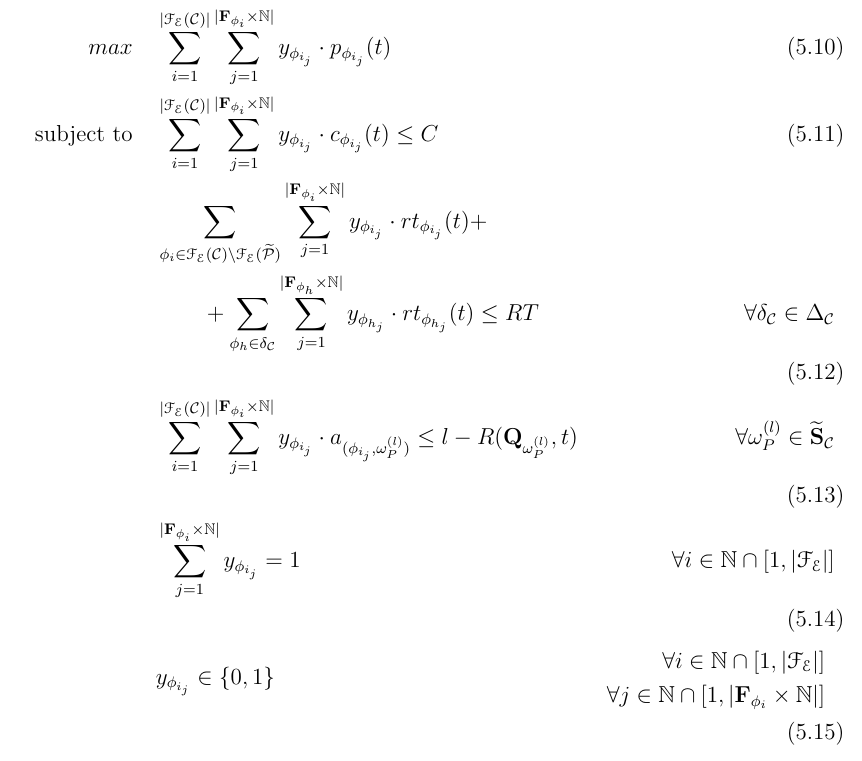
\includegraphics[width=\textwidth,height=0.8\columnwidth]{../Images/MMKPForSlide.png}
\end{figure}
	
	
\end{frame}



% -------------- %
% -------------- %
\begin{frame}{The Heuristic Algorithm}
	
	\begin{block}{}
		\centering
		The heuristic algorithm is based on \textit{Ant Colony Optimization} (ACO), a class of stochastic meta-heuristics: it is called Pre-provisioned Colony Optimization Algorithm with Lazy Pheromone Update
	\end{block}
	
	\begin{itemize}
		\item It is based on a set of computational agents, called \textit{artificial ants}, which \B{iteratively} construct a so-called \textit{partial solution}.
		
		\vspace{\baselineskip}
		
		\item At each iteration, each artificial ant moves from a partial solution to another, applying a series of stochastic local decisions whose policy is based on following parameters
		
		\begin{itemize}
			\item \textbf{Attractiveness}.
			\item \textbf{Pheromone Trail}.
		\end{itemize}
		
	\end{itemize}
	
	
	
	
\end{frame}
% -------------- %
% -------------- %
\begin{frame}{The Heuristic Algorithm}
	
	\begin{itemize}
		\item Lazy approach for pheromone trails update on the solution component graph.
		
		\item We exploit pre-provisioning tactic to anticipates data needs assuring a lower latency.
	\end{itemize}



\end{frame}
% -------------- %
% -------------- %
\begin{frame}
	
	\begin{figure}[h]
		\centering
		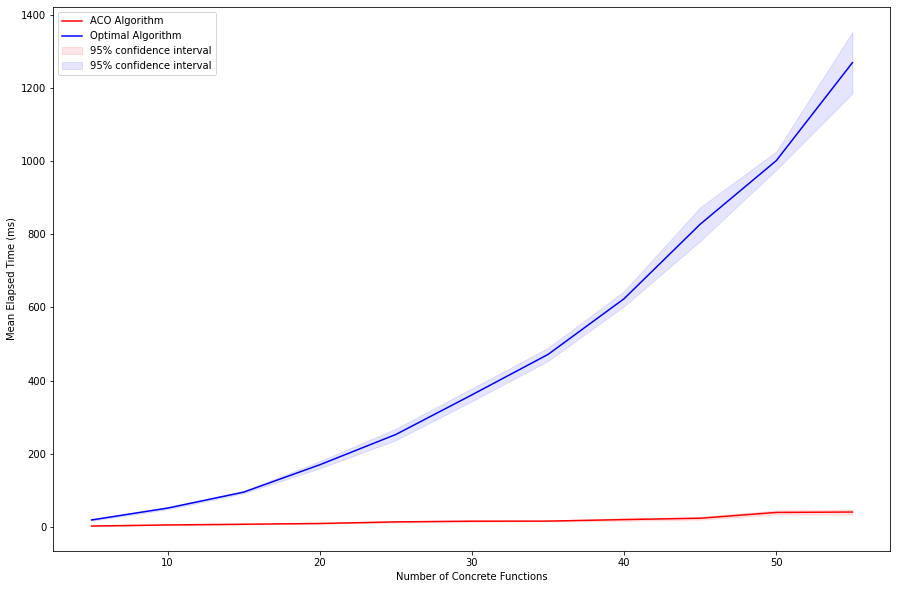
\includegraphics[width=\textwidth, height=0.8\textheight]{../Images/ACOvsOptimalIncreasingConcrete.png}
	\end{figure}
	
\end{frame}

% -------------- %
% -------------- %

\begin{frame}
	
	\begin{figure}[h]
		\centering
		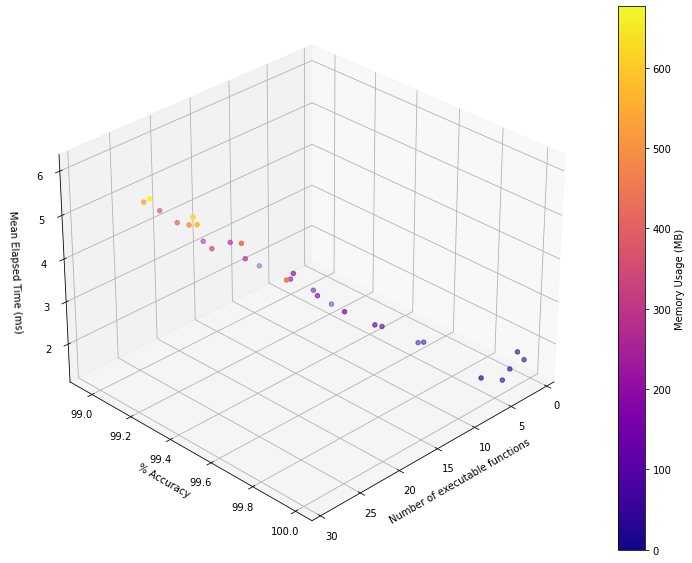
\includegraphics[width=\textwidth, height=0.8\textheight]{../Images/ACO3DIncreasingExecutable.png}
	\end{figure}
	
\end{frame}




\setbeamertemplate{background}{%
	\begin{tikzpicture}[overlay,remember picture]
		\node[scope fading=west,anchor=north west] at ([shift={(2in,-1in)}]current page.north west) {
\includegraphics[width=9cm,height=9cm]{../Images/UniLogo/TorVergataWatermark.png}};
	\end{tikzpicture}
}

\begin{frame}{{}}
	\begin{block}{}
		\centering
		Thanks for your attention!\\\B{Questions}?
	\end{block}
\end{frame} 

\end{document}
